\documentclass[border=10pt]{standalone}
\usepackage{tikz}
\usepackage{amsmath}

\begin{document}

% HCF Cross Section Figure
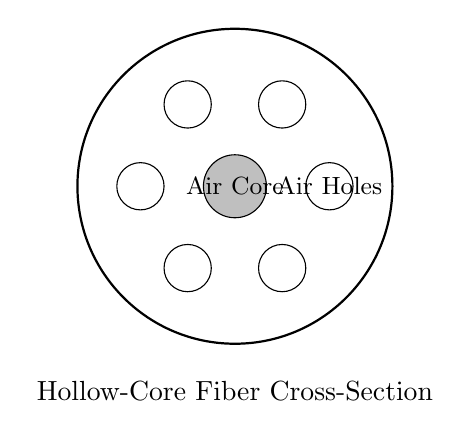
\begin{tikzpicture}[scale=2]
  % Outer cladding
  \draw[thick] (0,0) circle (1);
  % Air holes
  \foreach \angle in {0,60,120,180,240,300} {
    \draw[fill=white] (\angle:0.6) circle (0.15);
  }
  % Central air core
  \draw[fill=lightgray] (0,0) circle (0.2);
  
  % Labels
  \node at (0,0) {\small Air Core};
  \node at (0.6,0) {\small Air Holes};
  \node at (0,-1.3) {Hollow-Core Fiber Cross-Section};
\end{tikzpicture}

\end{document}
